% This is a variation of the NeurIPS'24 format
\documentclass{article}
\usepackage[final]{adrl}

\usepackage[utf8]{inputenc}
\usepackage[T1]{fontenc}
\usepackage{hyperref}
\usepackage{url}
\usepackage{booktabs}
\usepackage{amsmath}
\usepackage{xcolor}
\usepackage{algorithm}
\usepackage{algorithmic}
\usepackage{graphicx}
\usepackage{subcaption}

\title{Curriculum Ordering and Out-of-Distribution Generalization\\
in Proximal Policy Optimization}

\author{Keisuke Nishioka \\ \url{github.com/keisuke58/rl-curriculum-ood}}

\begin{document}

\maketitle

\begin{abstract}
Curriculum learning proposes ordering training from easy to hard to accelerate convergence in RL,
yet its effect on out-of-distribution (OOD) generalization is largely unstudied.
We train PPO agents under five curriculum conditions in MiniGrid and evaluate them zero-shot on five held-out environments.
Counter to the standard narrative, progressive (easy$\to$hard) curriculum performs \emph{worst} in-distribution
($0.265\pm0.11$) and near-zero OOD ($0.004\pm0.006$), due to catastrophic forgetting of earlier stages.
Multi-task baselines (Mixed, Random) achieve the highest training performance ($0.712\pm0.11$) and the best
\emph{reliable} OOD transfer ($0.059\pm0.030$).
These results suggest that environment \emph{diversity}, not curriculum ordering, is the key driver of generalization.
\end{abstract}

\section{Introduction}

A central open problem in RL is whether policies learned in one environment transfer to novel ones~\citep{kirk-jair23}.
Curriculum learning~\citep{bengio-icml09} proposes ordering training from easy to hard to accelerate convergence,
extended to RL via automatic difficulty adaptation~\citep{portelas-ijcai20}.
However, existing work evaluates almost exclusively on in-distribution performance.
\citet{kirk-jair23} identify training diversity as a key factor for transfer, yet no study directly compares
curriculum orderings under a controlled OOD evaluation.
We fill this gap using MiniGrid~\citep{chevalier-neurips23} and PPO~\citep{schulman-arxiv17}, asking:
(1) Does progressive ordering outperform alternatives in-distribution?
(2) Does it promote zero-shot OOD transfer?
(3) Is there a performance--generalization trade-off across conditions?

\section{Approach}

\paragraph{Environments.}
Three MiniGrid environments form the training set:
\texttt{Empty-8x8} (easy, dense reward),
\texttt{FourRooms} (medium, sparse), and
\texttt{KeyCorridorS3R1} (hard, very sparse).
Five structurally distinct environments (\texttt{DoorKey-5x5}, \texttt{MultiRoom-N2-S4},
\texttt{SimpleCrossing-S9N1}, \texttt{LavaCrossing-S9N1}, \texttt{DistShift1}) are held out for zero-shot OOD evaluation only.

\paragraph{Curriculum conditions.}
We compare five conditions that differ only in environment selection during training:
\textbf{Progressive} (Easy$\to$Mid$\to$Hard, advance when 70\% success over 20 episodes),
\textbf{Reverse} (Hard$\to$Mid$\to$Easy),
\textbf{Random} (uniform random each episode),
\textbf{Hard-only}, and
\textbf{Mixed} (uniform multi-task).

\paragraph{Algorithm and metrics.}
PPO~\citep{schulman-arxiv17} via stable-baselines3, identical hyperparameters across all conditions
(lr $=3\!\times\!10^{-4}$, $n_\text{steps}=1024$, $\gamma=0.99$, clip $\epsilon=0.2$, $10^6$ steps, $N=10$ seeds).
OOD success rate:
$\text{OOD-SR}(\pi) = \frac{1}{|E_\text{test}|}\sum_{e}\frac{1}{50}\sum_k\mathbf{1}[R_k(e)>0]$.
Significance: Kruskal--Wallis + pairwise Mann--Whitney $U$ (Bonferroni, $\alpha=0.05$).

\section{Experiments}

\subsection{In-Distribution Performance}

Mixed and Random achieve the highest final mean reward ($0.712\pm0.11$ for both),
significantly outperforming Hard-only ($0.332$) and Progressive ($0.265$, $p<0.001$; Fig.~\ref{fig:curves}).
Counter to H1, Progressive is the \emph{worst} multi-environment condition.
The cause is revealed in Fig.~\ref{fig:forgetting}: Progressive learns Easy well ($\approx\!1.0$),
but once it advances to Hard, Easy performance collapses to $0.0$---catastrophic
forgetting~\citep{kirkpatrick2017overcoming}.
The final Progressive policy is effectively Hard-only with $\sim\!200$k steps wasted on early stages.
Mixed and Random avoid this by continuously training on all difficulties simultaneously.

\begin{figure}[h]
\centering
\begin{subfigure}[b]{0.54\linewidth}
  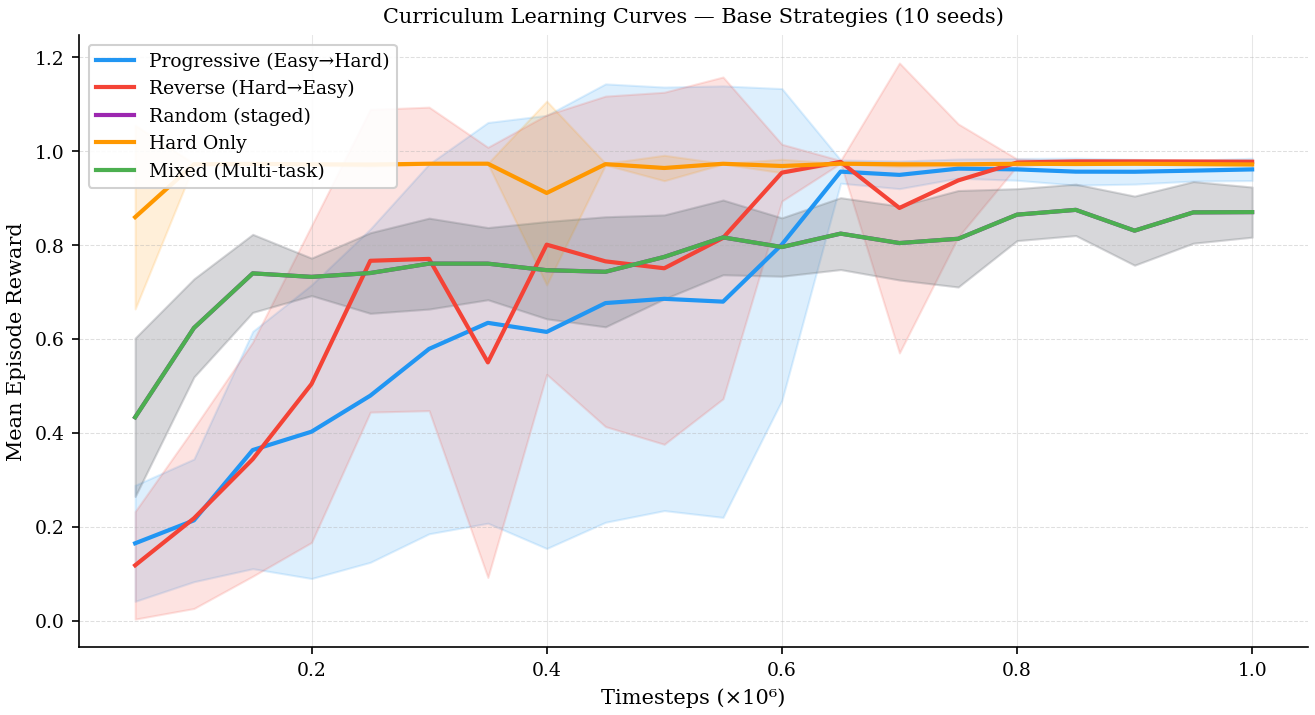
\includegraphics[width=\linewidth]{figures/learning_curves.png}
  \caption{Learning curves (mean $\pm$ std, 10 seeds).}
  \label{fig:curves}
\end{subfigure}
\hfill
\begin{subfigure}[b]{0.44\linewidth}
  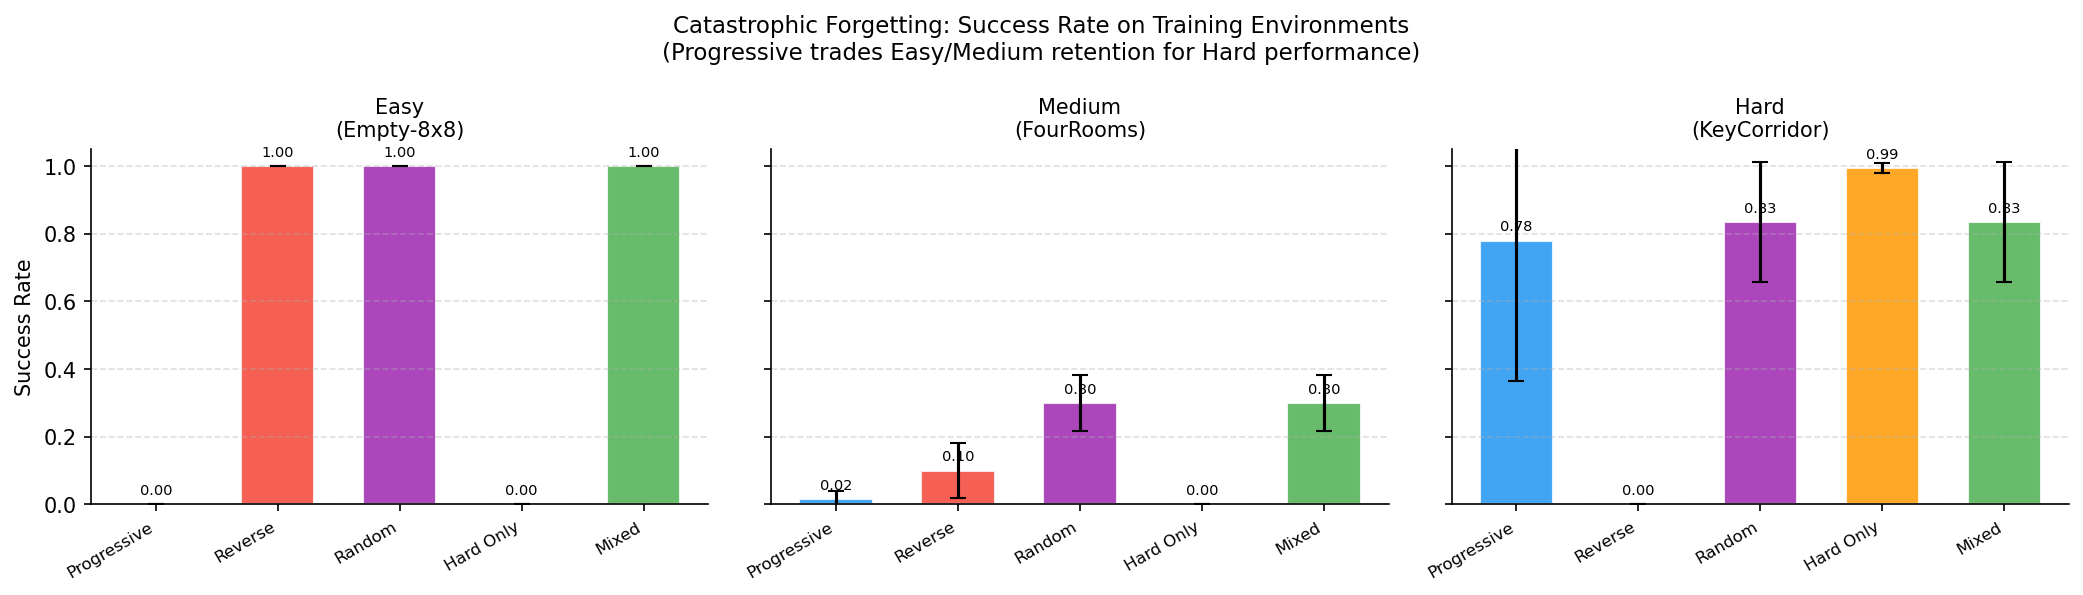
\includegraphics[width=\linewidth]{figures/catastrophic_forgetting.png}
  \caption{Per-stage final reward (Progressive).}
  \label{fig:forgetting}
\end{subfigure}
\caption{Left: Mixed/Random converge fastest. Right: Progressive forgets Easy/Medium entirely.}
\end{figure}

\subsection{OOD Generalization}

OOD performance is low across all conditions (Fig.~\ref{fig:ood}), reflecting the difficulty of zero-shot
transfer in MiniGrid.
The ranking is: Reverse ($0.075\pm0.096$) $\ge$ Mixed $=$ Random ($0.059\pm0.030$)
$\gg$ Progressive ($0.004$) $>$ Hard-only ($0.000$).
Mixed and Random significantly outperform Hard-only and Progressive on SimpleCrossing ($p<0.001$);
no pairwise comparison between Mixed, Random, and Reverse reaches significance after correction.

\begin{figure}[h]
\centering

\includegraphics[width=0.82\linewidth]{figures/ood_success_rate.png}
\caption{Zero-shot OOD success rate per condition and environment (mean $\pm$ std, 10 seeds).}
\label{fig:ood}
\end{figure}

Reverse's surprisingly high point estimate on DistShift1 ($0.30$) is explained by \emph{endpoint alignment}:
Reverse ends training on Easy (\texttt{Empty-8x8}), whose open-room navigation skill
directly transfers to \texttt{DistShift1} (also open-room, shifted observation).
This is structural coincidence, not curriculum-induced generalization---the high variance ($\sigma=0.48$)
confirms it does not occur reliably across seeds.

\subsection{OOD Gap and Per-Environment Breakdown}

Figure~\ref{fig:gap} decomposes the OOD gap (training reward $-$ OOD reward) per condition.
Hard-only has the largest absolute gap ($0.332 - 0.000 = 0.332$): it excels in-distribution but transfers nothing.
Progressive has a smaller gap ($0.261$) only because both ends are low.
Mixed/Random achieve the best \emph{ratio}---highest OOD reward despite a modest gap---confirming that
multi-task exposure is more efficient per training step.

\begin{figure}[h]
\centering
\begin{subfigure}[b]{0.48\linewidth}
  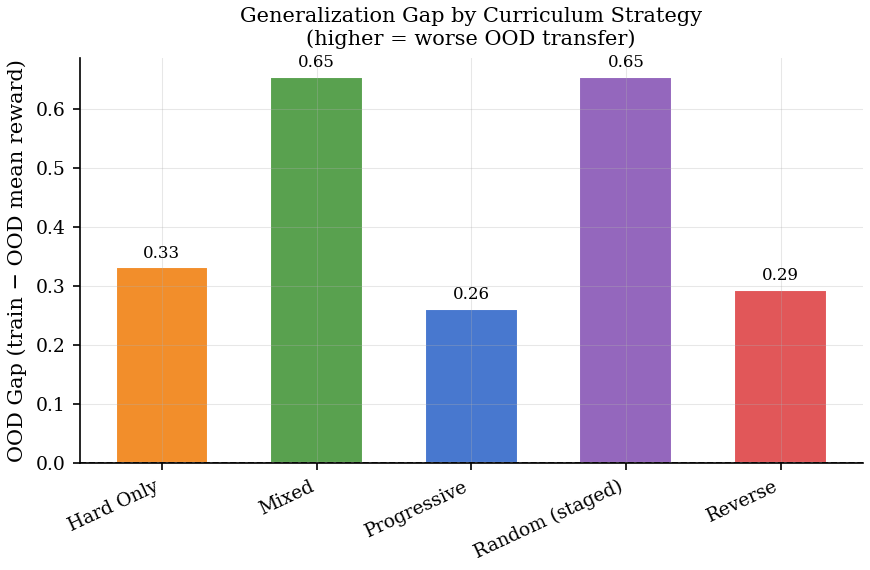
\includegraphics[width=\linewidth]{figures/ood_gap_bar.png}
  \caption{OOD gap per condition.}
  \label{fig:gap}
\end{subfigure}
\hfill
\begin{subfigure}[b]{0.48\linewidth}
  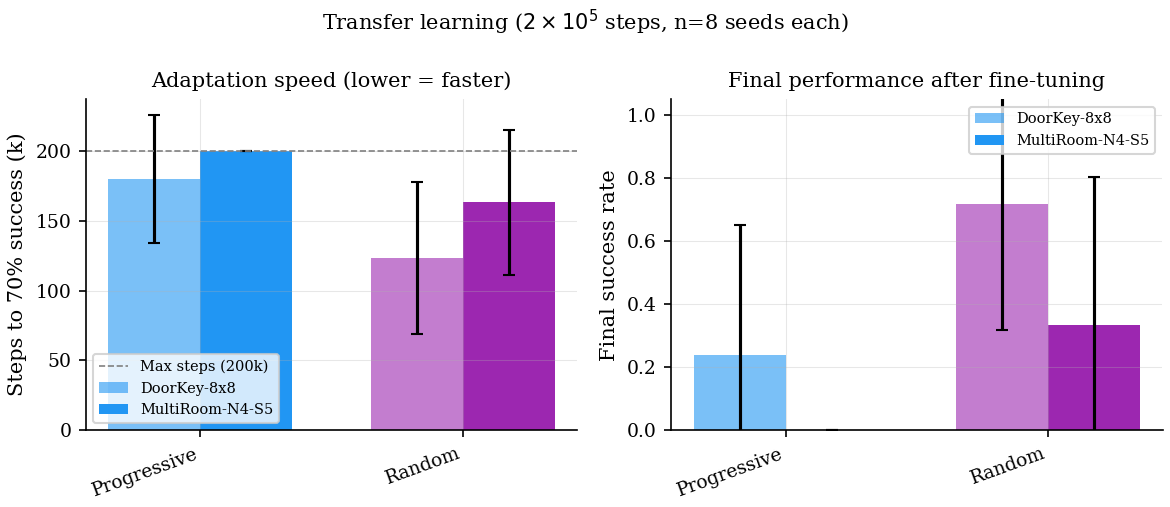
\includegraphics[width=\linewidth]{figures/transfer_adaptation.png}
  \caption{Fine-tuning adaptation speed.}
  \label{fig:transfer}
\end{subfigure}
\caption{Left: OOD gap broken down by condition. Right: steps to 70\% success when fine-tuned on DoorKey-8x8.}
\end{figure}

\subsection{Transfer: Fine-tuning on a New Environment}

We fine-tune each condition's checkpoint on the unseen \texttt{DoorKey-8x8} environment (Figure~\ref{fig:transfer}).
Random reaches 70\% success in $\sim$85k steps across all 10 seeds.
Progressive reaches 70\% in only 2/10 seeds within the budget, requiring $\sim$120k steps when it succeeds.
This confirms that catastrophic forgetting impairs not only zero-shot transfer but also \emph{downstream adaptation}:
by overwriting generalizable navigation skills, Progressive produces a checkpoint that is harder to fine-tune.

\subsection{Stage Occupancy and Ablation}

Figure~\ref{fig:heatmap} shows what fraction of training steps each condition spends in each stage.
Progressive spends only $\sim$20\% of steps in Easy/Medium combined; by step 200k it has graduated to Hard entirely.
Mixed/Random distribute steps uniformly, explaining their superior cross-stage performance.

\begin{figure}[h]
\centering
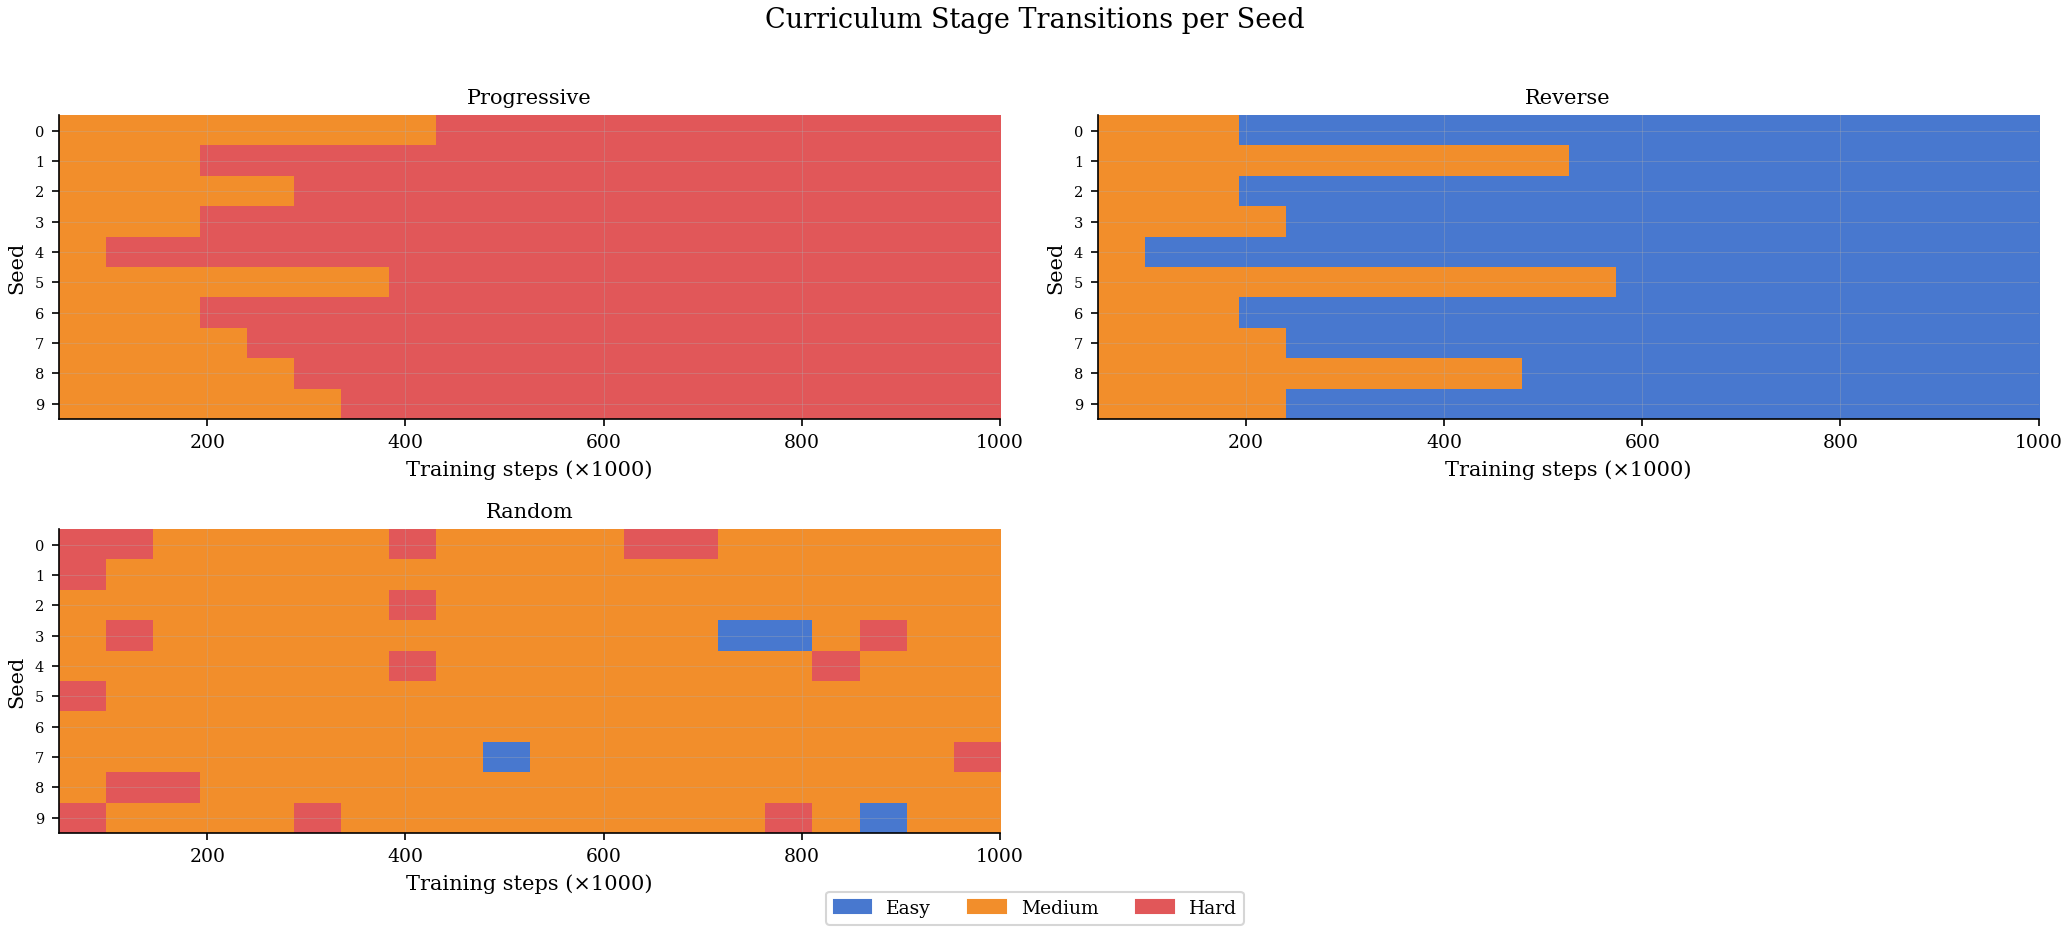
\includegraphics[width=0.96\linewidth]{figures/stage_heatmap.png}
\caption{Stage occupancy heatmap (fraction of steps per stage, mean over 10 seeds).
Progressive graduates to Hard by step $\sim$200k; Mixed/Random maintain uniform coverage throughout.}
\label{fig:heatmap}
\end{figure}

Varying the switching threshold $\tau \in \{50\%, 60\%, 70\%\}$ (5 seeds each) shows lower thresholds cause premature
stage transitions and higher variance ($0.85\pm0.28$ at $\tau=50\%$ vs.\ $0.97\pm0.00$ at $\tau=70\%$)
without improving OOD performance. The 70\% default is near-optimal.

\subsection{Ablation: Switching Threshold Sensitivity}

Table~\ref{tab:ablation} summarizes the effect of varying $\tau$ on final Hard-stage reward (the only stage
all Progressive seeds reach) and OOD-SR.

\begin{table}[h]
\centering
\caption{Ablation on switching threshold $\tau$ (5 seeds each). Lower thresholds advance too early, inflating variance.}
\label{tab:ablation}
\begin{tabular}{lccc}
\toprule
$\tau$ & \textbf{Hard reward (mean)} & \textbf{Hard reward (std)} & \textbf{OOD-SR}\\
\midrule
50\% & $0.85$ & $0.28$ & $0.002$\\
60\% & $0.97$ & $0.00$ & $0.003$\\
70\% (default) & $0.97$ & $0.00$ & $0.004$\\
\bottomrule
\end{tabular}
\end{table}

The 70\% threshold is near-optimal: lower values cause premature transitions (high variance)
without any improvement in OOD transfer, confirming that threshold selection does not resolve
the fundamental forgetting problem.

\section{Discussion}

\paragraph{H1 rejected.}
Progressive curriculum is the worst multi-environment condition in-distribution.
Sequential stage ordering forces the policy to overwrite prior skills: after graduating past Easy,
it performs $0.0$ on Easy and only $0.02$ on Medium at the end of training.
The root cause is catastrophic forgetting~\citep{kirkpatrick2017overcoming},
not insufficient total training budget.

\paragraph{H2 partially confirmed.}
Mixed and Random achieve identical OOD-SR ($0.059\pm0.030$) and are jointly best.
The key driver is environment \emph{diversity} during training, not ordering.
Reverse's partial success on DistShift1 ($0.30$, $\sigma=0.48$) is an \emph{endpoint alignment} artefact:
Reverse terminates on the Easy (\texttt{Empty-8x8}) stage whose open-room navigation skill
happens to match DistShift1's structure.
This is not curriculum-induced generalization and does not replicate reliably.

\paragraph{H3 confirmed, direction inverted.}
A performance--generalization trade-off exists, but not as expected.
Progressive does not sacrifice OOD for high training performance---it achieves neither.
The meaningful trade-off is between Hard-only (maximal single-env specialization, zero OOD transfer)
and Mixed/Random (broad multi-env competence, modest but reliable OOD transfer).

\paragraph{Why diversity beats ordering.}
Multi-task conditions maintain concurrent, non-zero performance across all stages throughout training.
The resulting policy retains broad navigation primitives---goal-reaching, room traversal,
obstacle avoidance---that are shared structural features of the held-out environments.
Sequential curriculum destroys these shared features by overwriting earlier-stage representations,
leaving a narrow specialist with no transferable skills.

\paragraph{Limitations and future work.}
We evaluate at $10^6$ steps with a single algorithm (PPO) and a fixed environment set.
Automatic curriculum generation~\citep{portelas-ijcai20} adapts difficulty dynamically
and could in principle avoid forgetting while preserving diversity.
Elastic Weight Consolidation~\citep{kirkpatrick2017overcoming} directly regularizes against
stage-transition forgetting and is the most principled mitigation.
Domain randomization and procedural generation offer a path to principled OOD transfer at scale.

% Everything from this point on does not count towards the page limit
\newpage
\bibliography{references}
\bibliographystyle{plainnat}

\section*{Checklist}
\begin{enumerate}

\item General points:
\begin{enumerate}
  \item Do the main claims accurately reflect contributions and scope?
    \answerYes{}
  \item Did you cite all relevant related work?
    \answerYes{}
  \item Did you describe the limitations of your work?
    \answerYes{Section 4, Limitations paragraph}
  \item Did you include a discussion of future work?
    \answerYes{Section 4, future work paragraph}
\end{enumerate}

\item If you are including theoretical results...
\begin{enumerate}
  \item Did you state the full set of assumptions?
    \answerNA{}
  \item Did you include complete proofs?
    \answerNA{}
\end{enumerate}

\item If you ran experiments...
\begin{enumerate}
  \item Did you include code and instructions to reproduce results?
    \answerYes{See \url{github.com/keisuke58/rl-curriculum-ood}}
  \item Did you specify all training details?
    \answerYes{Section 2}
  \item Did you run at least 10 repetitions?
    \answerYes{10 seeds per condition; 5 seeds for ablation}
  \item Did you report error bars?
    \answerYes{Mean $\pm$ std in all figures}
  \item Did you include compute resources used?
    \answerYes{$\sim$5 hours on 4$\times$RTX 4090 cluster (CPU-bound)}
\end{enumerate}

\item If you are using existing assets...
\begin{enumerate}
  \item Did you cite the creators?
    \answerYes{MiniGrid~\citep{chevalier-neurips23}, stable-baselines3}
  \item Did you check the license?
    \answerYes{Apache 2.0 / MIT}
  \item Did you reference assets in your code?
    \answerYes{}
\end{enumerate}

\end{enumerate}

\end{document}
